\subsection{Диаграмма развертывания}

UML диаграмма развертывания (англ.deployment diagram) является визуальным инструментом,
применяемым для моделирования физической конфигурации системы и ее компонентов.
Ее цель состоит в описании распределения аппаратных и программных ресурсов,
а также связей между ними.
На рисунке~\ref{fig:db_UML_deployment_mobile} представлена UML-диаграмма развертывания,
созданная в контексте разработки мобильного приложения.

% UML-диаграмма развертывания (англ. deployment diagram) — это графическое представление,
% которое используется для моделирования физической конфигурации системы и ее компонентов.
% Она позволяет описать распределение аппаратных и программных ресурсов, а также взаимосвязи между ними.

% Диаграмма развертывания помогает визуализировать, как компоненты системы размещаются на аппаратных устройствах,
% а также как они связаны между собой через сети и каналы связи.
% Эта диаграмма предоставляет общую картину физического размещения системы и ее взаимодействия с окружающей средой.

% UML Диаграмма развертывания при разработке мобильного приложения изображена на рисунке~\ref{fig:db_UML_deployment_mobile}.

\begin{figure}[!h]
    \centering

    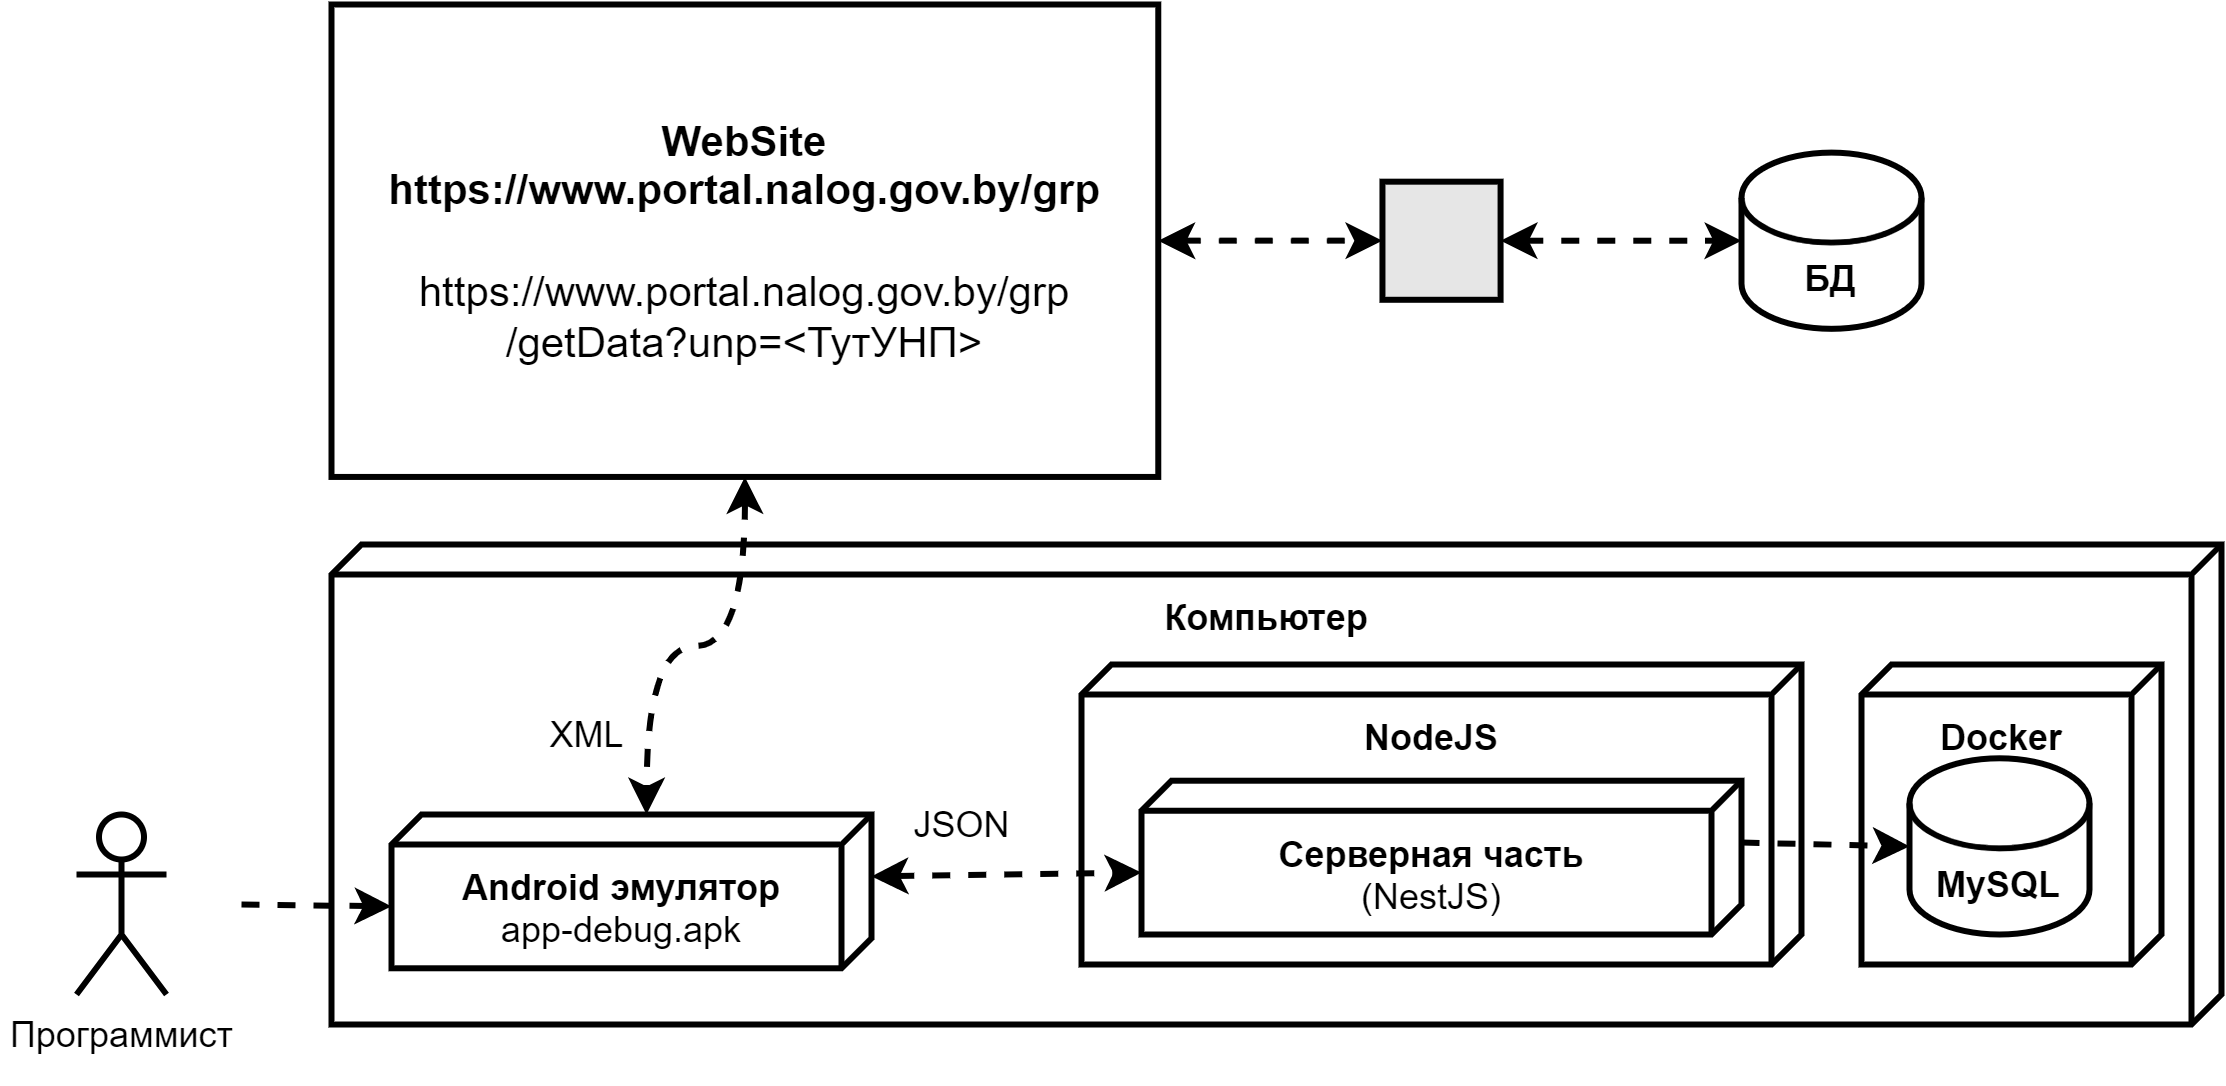
\includegraphics[width=14cm]
    {images/UML/deployment/mobile.png}

    \caption{UML диаграмма развертывания работы мобильного приложения}

    \label{fig:db_UML_deployment_mobile}
\end{figure}

На рисунке~\ref{fig:db_UML_deployment_admin} изображена UML диаграмма развертывания для панели администратора.
Панель менеджера использует такие же технологии, а именно библиотеку ReactJS (create-react-app) на языке программирования TypeScript,
как и панель администратора.
Диаграмма развертывания для панели менеджера будет аналогична диаграмме развертывания для панели администратора.

\begin{figure}[!h]
    \centering

    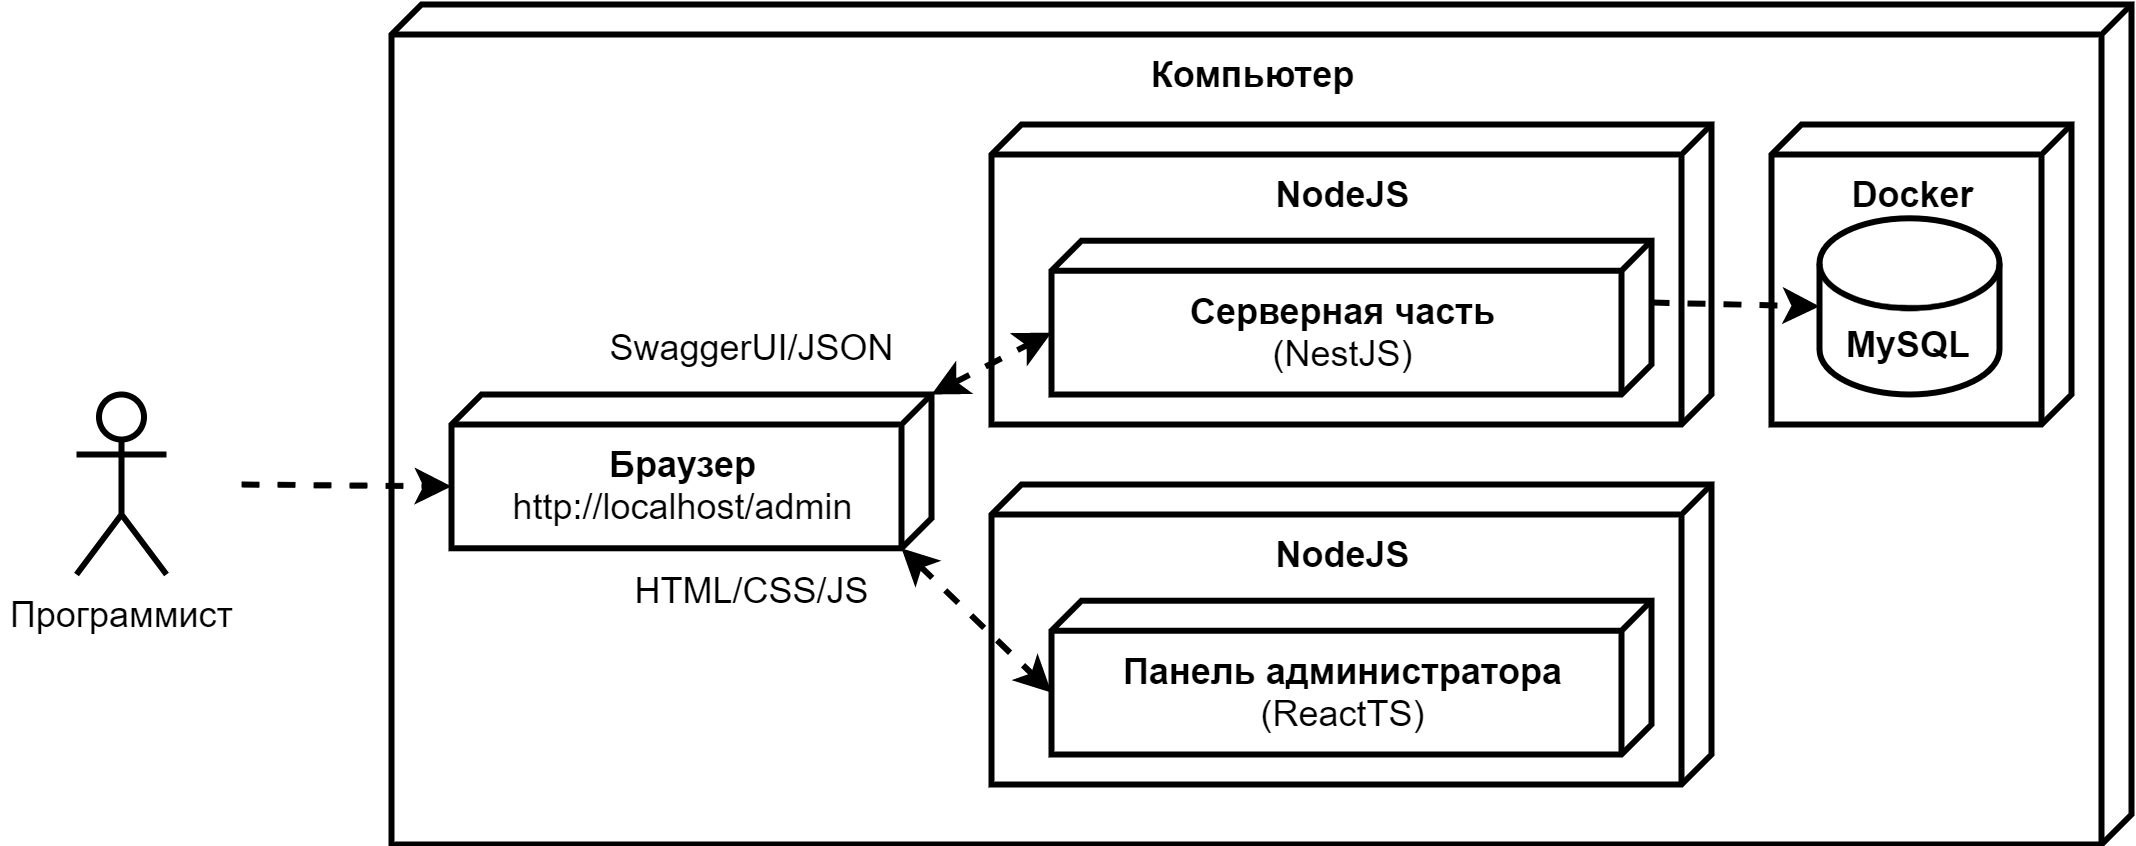
\includegraphics[width=13cm]
    {images/UML/deployment/admin.png}

    \caption{UML диаграмма развертывания для панели администратора}

    \label{fig:db_UML_deployment_admin}
\end{figure}

Для запуска системы глобально можно воспользоваться панелью управления веб-хостингом cPanel,
доступной для приобретения у Login.by, а чтобы не использовать IP машины, купить домен у Hoster.by.
Login.by предоставляет возможность ознакомления с cPanel в течении семи дней,
а затем, в случае удовлетворения, можно произвести оплату.

На веб-хостинге cPanel, доступна база данных MySQL, что позволит хранить данные не на своем компьютере.
Также можно запускать NodeJS приложения, что обеспечит работу нашей серверной части (backend).

Так как база данных пуста, то необходимо выполнить миграции, чтобы создать необходимые таблицы в базе данных.
После этого можно запустить серверную часть (backend).

В cPanel также имеется веб-сервер Apache, на котором можно разместить файлы HTML/CSS/JS,
полученные в результате сборки приложения с использованием create-react-app.
Таким образом, можно развернуть панель администратора (frontend) и панель менеджера (frontend).
Мобильно приложение (frontend) нужно распостранять как apk-файл, например, через сайт или Play Market.

UML диаграмма развертывани для системы,
которая использует панель управления веб-хостингом cPanel изображена на рисунке~\ref{fig:db_UML_deployment_prod}.

\begin{figure}[!h]
    \centering

    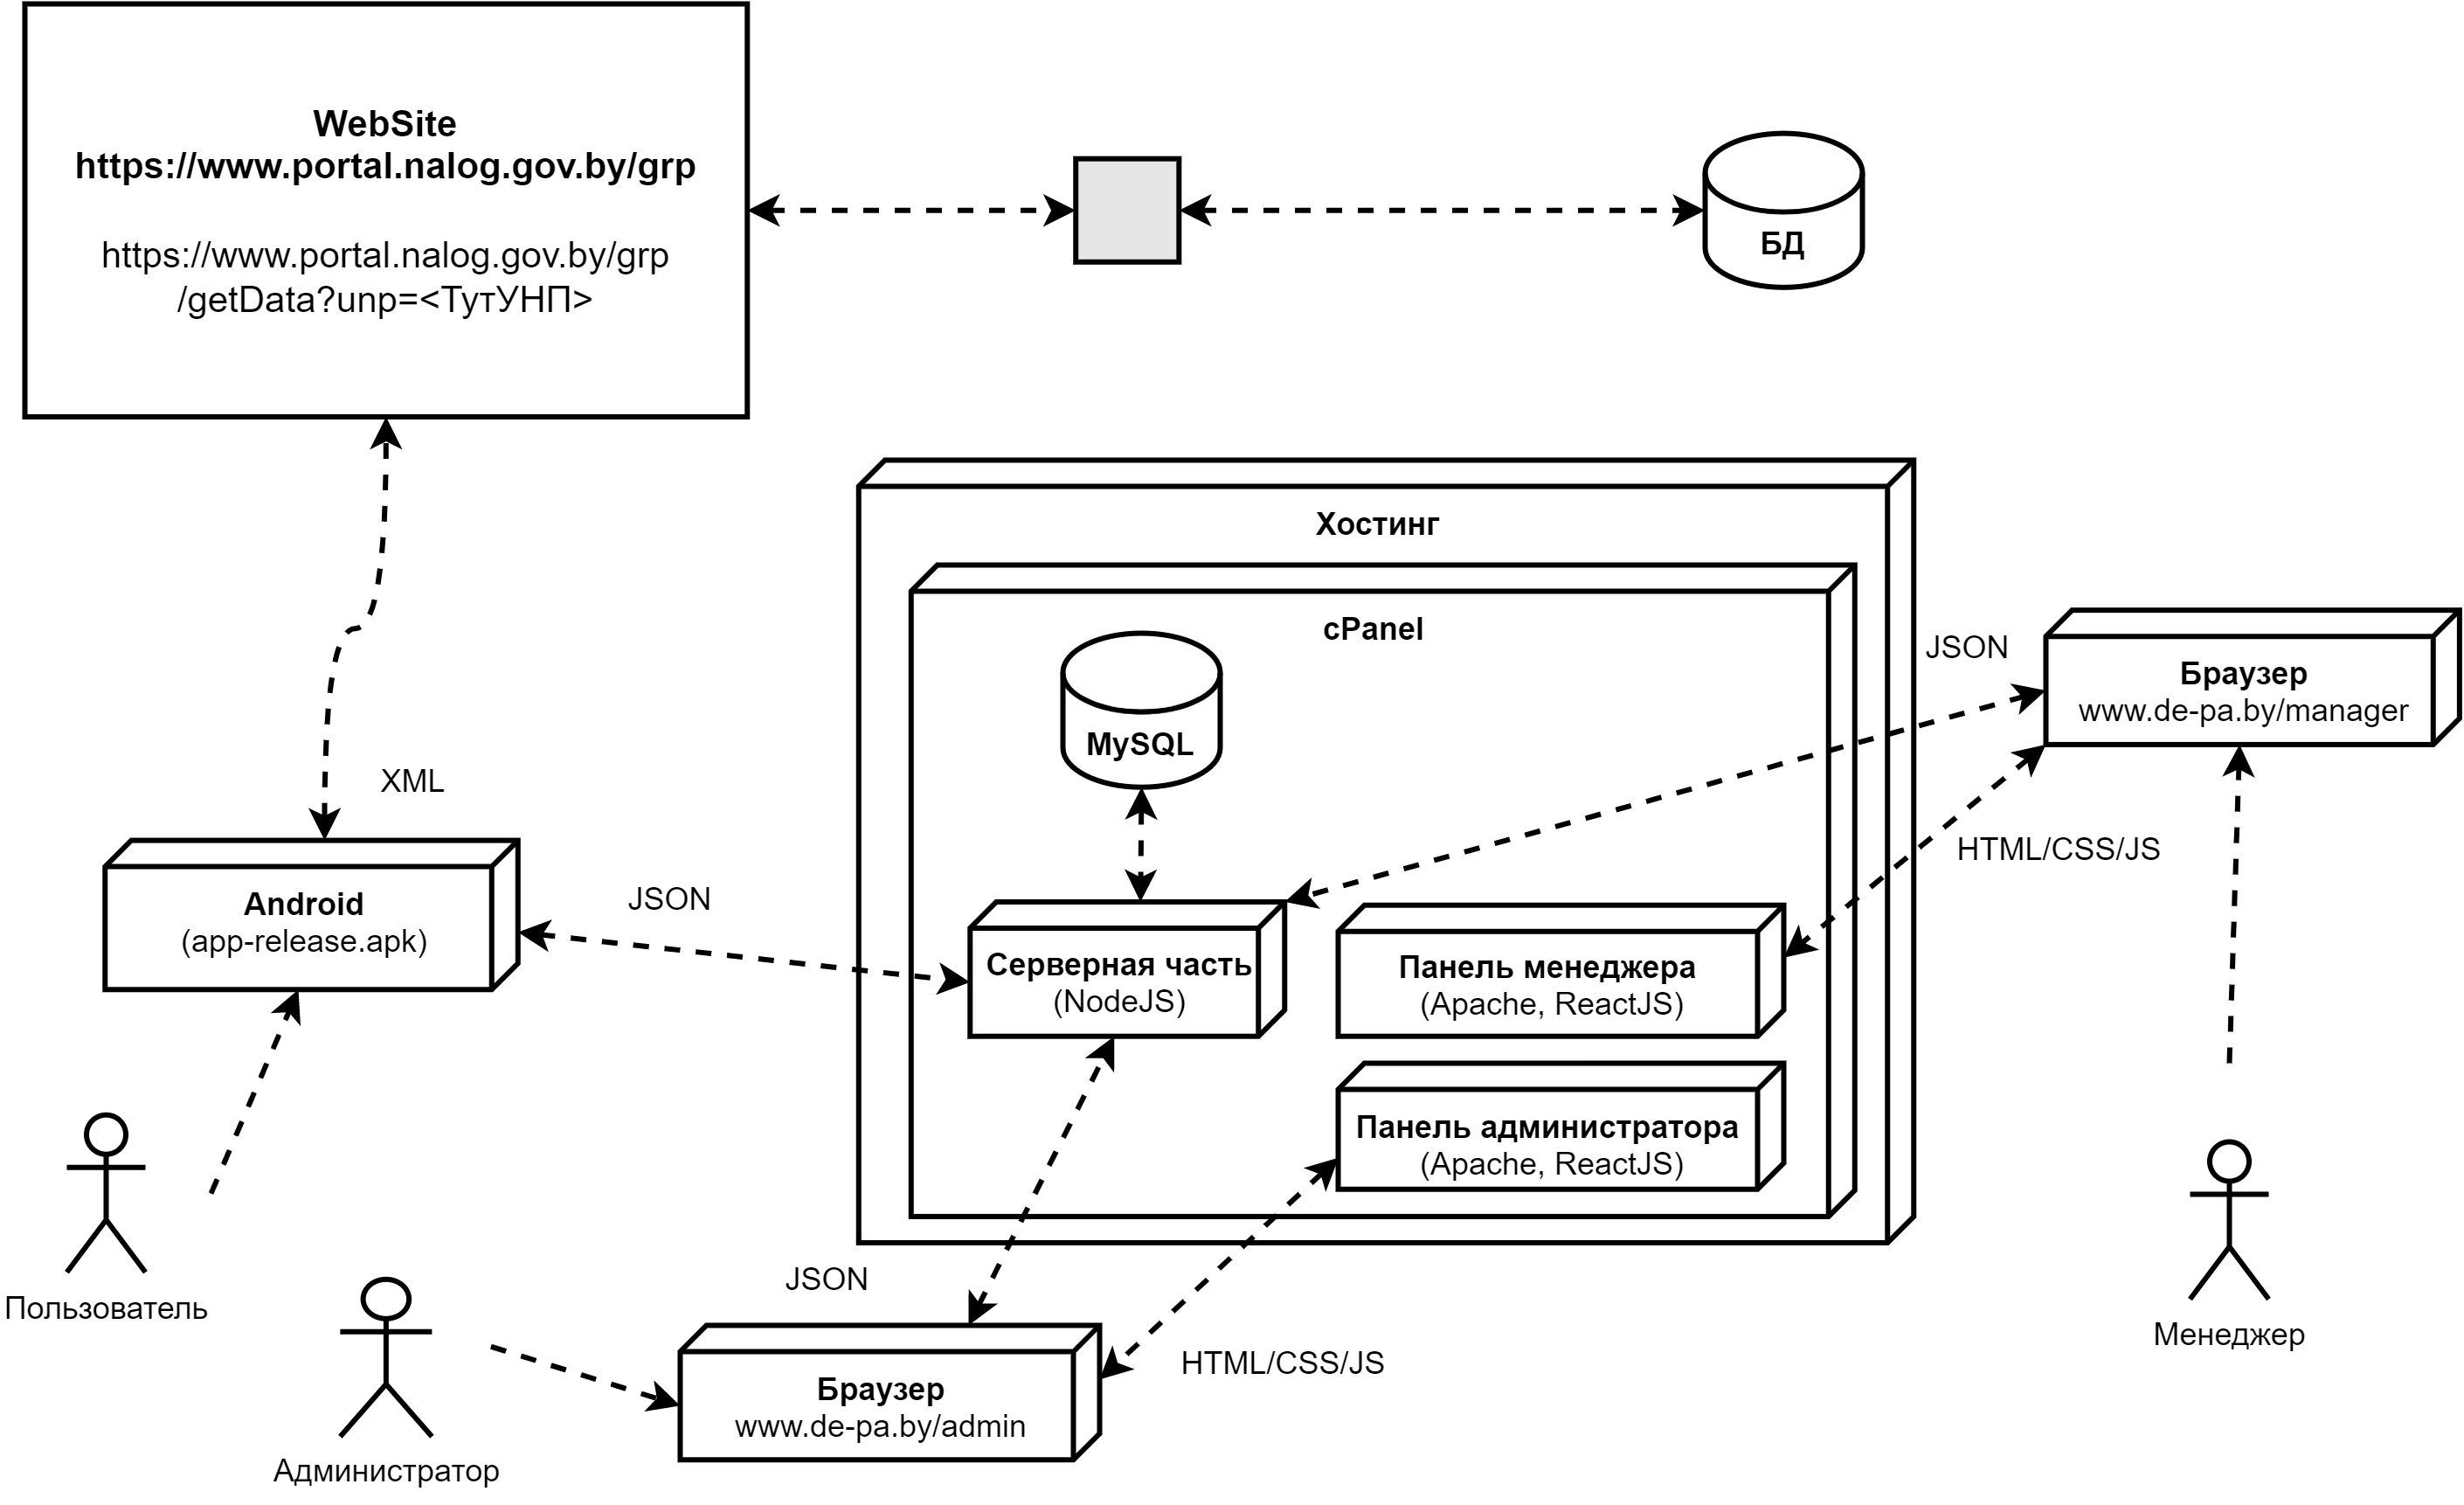
\includegraphics[width=15cm]
    {images/UML/deployment/production_no_comment.png}

    \caption{UML диаграмма развертывания в глобальной сети}

    \label{fig:db_UML_deployment_prod}
\end{figure}
